\documentclass{article}

% Useful packages
\usepackage[dutch]{babel} % Nederlands taalpakket
\usepackage{multicol}
\setlength{\columnsep}{1cm}

% Set page size and margins
% Replace `letterpaper' with `a4paper' for UK/EU standard size
\usepackage[a4paper,top=2cm,bottom=2cm,left=2cm,right=2cm,marginparwidth=1.75cm]{geometry}

\usepackage{amsmath}
\usepackage{siunitx}
\usepackage{wrapfig}
\usepackage{float}
\usepackage{graphicx}
\graphicspath{{images/}}
\usepackage{subcaption}
\usepackage[colorlinks=true, allcolors=blue]{hyperref}
\usepackage{xcolor}
\usepackage{listings}
\usepackage{import}
\usepackage{xcolor}
\usepackage[toc,page]{appendix} % Pakket voor het maken van bijlagen
\usepackage{hyperref} % Pakket voor hyperlinks en verwijzingen
\usepackage{rotating}
\usepackage{array}
\usepackage{multirow}
\usepackage{lscape}
\usepackage{pdflscape}
\usepackage{longtable} % Add the longtable package to define the longtable environment
\usepackage{caption} % Add the caption package to use the \caption command
\usepackage{etex} % Add the etex package to use the \reserveinserts command


% Definieer de kleuren voor syntax highlighting
\definecolor{codegreen}{rgb}{0,0.6,0}
\definecolor{codegray}{rgb}{0.5,0.5,0.5}
\definecolor{codepurple}{rgb}{0.58,0,0.82}
\definecolor{backcolour}{rgb}{0.95,0.95,0.92}



\lstdefinestyle{mystyle}{
    backgroundcolor=\color{backcolour},
    commentstyle=\color{codegreen},
    keywordstyle=\color{codepurple},
    numberstyle=\tiny\color{codegray},
    basicstyle=\footnotesize\ttfamily,
    breakatwhitespace=false,
    breaklines=true,
    captionpos=b,
    keepspaces=true,
    numbers=left,
    numbersep=5pt,
    showspaces=false,
    showstringspaces=false,
    showtabs=false,
    tabsize=2
}

\usepackage[dutch]{babel}% Language setting


\title{
    Life Cycle Engineering \\
    \large Uitvoeren van safety/reliability analyse}

\author{
  Vollmuller, Michel\\
  1809572\\
  \texttt{michel.vollmuller@student.hu.nl}
} 

\begin{document}
\maketitle

% \begin{abstract}
% \end{abstract}

\tableofcontents

\newpage
\section{Inleiding}


\newpage
\section{Opdrachtomschrijving}



\newpage
\section{Functioneel Schema}

\begin{figure}[H]
  \centering
  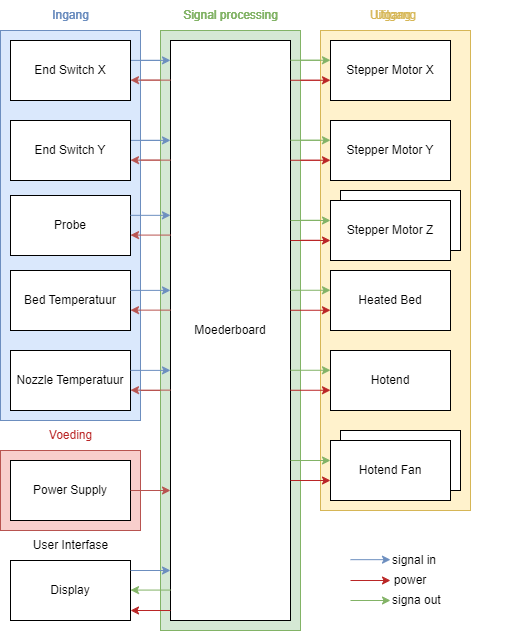
\includegraphics[width=\textwidth]{Creality Ender V2.drawio.png}
\end{figure}


\newpage
\section{FMEA}
\setlength{\parindent}{0pt} % No indentation for new paragraphs
\subsection{scope}
De scope van deze FMEA is gericht op de elektrische componenten van de Creality Ender 3 V2 3D-printer. Een FMEA (Failure Mode and Effects Analysis) is een methode om potentiële faalmodi, hun effecten en de ernst ervan te identificeren. In dit geval richten we ons specifiek op de elektrische componenten van de printer, zoals de voeding, eindschakelaars, bed temperatuur, probe, moederbord, stepper motoren, verwarmd bed, hotend en hotend ventilator.

Het doel van deze FMEA is om potentiële faalmodi in de elektrische componenten van de 3D-printer te identificeren en de ernst van de effecten te beoordelen. Door deze analyse uit te voeren, kunnen we proactieve maatregelen nemen om de betrouwbaarheid en veiligheid van de printer te verbeteren. Dit kan bijvoorbeeld leiden tot het implementeren van redundante systemen, het verbeteren van de detectie van storingen of het nemen van corrigerende acties om de risico's te verminderen.

Het resultaat van deze FMEA is een tabel waarin de verschillende faalmodi, effecten, ernst, frequentie van optreden, detectie en risicoprioriteitsgetal (RPN) worden geëvalueerd. Op basis van deze evaluatie kunnen corrigerende acties worden voorgesteld om de risico's te verminderen en de betrouwbaarheid van de elektrische componenten te verbeteren.
\\
Deze FMEA is van belang voor het waarborgen van de kwaliteit en betrouwbaarheid van de Creality Ender 3 V2 3D-printer. Door potentiële faalmodi en hun effecten te identificeren, kunnen we proactief maatregelen nemen om storingen te voorkomen en de gebruikerservaring te verbeteren.

\subsection{Onderdelen}
\subsubsection*{End Switches}
% \cite{reddit_end_switches}

\subsubsection*{Bed Temperatuur}
% \cite{reddit_limit_switches}

\newpage
\begin{landscape}
    \subsection{FMEA Table} 
    \begin{longtable}{|l|l|l|c|c|c|c|l|}
        \hline
        \textbf{Item/Functie} & \textbf{Failure mode} & \textbf{Effect} & \textbf{Severity} & \textbf{Occurrence} & \textbf{Detection} & \textbf{RPN} & \textbf{Corr. Action} \\ \hline
        \multirow{3}{*}{Power Supply}       & Defect            & Geen voeding  & 2 & 2 & 5 & 20 & \\
                                            & Kortsluiting      & Geen voeding  & 2 & 2 & 1 &  4 & \\
                                            & Onderbreking      & Geen voeding  & 3 & 2 & 5 & 30 & TE HOOG \\
                                            \hline
        \multirow{4}{*}{End Switch X}       & Sensor defect     & X Switch low  & 2 & 2 & 5 & 20 & \\
                                            & Geen voeding      & X Switch low  & 2 & 2 & 1 &  4 & \\
                                            & false true        & X Switch high & 3 & 2 & 5 & 30 & TE HOOG \\
                                            & false false       & X Switch low  & 2 & 2 & 4 & 16 & \\ 
                                            \hline
        \multirow{4}{*}{End Switch Y}       & Sensor defect     & Y Switch low  & 2 & 2 & 5 & 20 & \\
                                            & Geen voeding      & Y Switch low  & 2 & 2 & 1 &  4 & \\
                                            & false true        & Y Switch high & 3 & 2 & 5 & 30 & TE HOOG \\
                                            & false false       & Y Switch low  & 2 & 2 & 4 & 16 & \\ 
                                            \hline
        \multirow{4}{*}{Probe}              & Sensor defect     & Probe low  & 2 & 2 & 5 & 20 & \\
                                            & Geen voeding      & Probe low  & 2 & 2 & 1 &  4 & \\
                                            & false true        & Probe high & 3 & 2 & 5 & 30 & TE HOOG \\
                                            & false false       & Probe low  & 2 & 2 & 4 & 16 & \\ 
                                            \hline
        \multirow{4}{*}{Bed Temperatuur}    & Sensor defect     & Bed Temperatuur low  & 2 & 2 & 5 & 20 & \\
                                            & Geen voeding      & Bed Temperatuur low  & 2 & 2 & 1 &  4 & \\
                                            & false true        & Bed Temperatuur high & 3 & 2 & 5 & 30 & TE HOOG \\
                                            & false false       & Bed Temperatuur low  & 2 & 2 & 4 & 16 & \\ 
                                            \hline
        \multirow{4}{*}{Nozzle Temperatuur} & Sensor defect     & Nozzle Temperatuur low  & 2 & 2 & 5 & 20 & \\
                                            & Geen voeding      & Nozzle Temperatuur low  & 2 & 2 & 1 &  4 & \\
                                            & false true        & Nozzle Temperatuur high & 3 & 2 & 5 & 30 & TE HOOG \\
                                            & false false       & Nozzle Temperatuur low  & 2 & 2 & 4 & 16 & \\ 
                                            \hline          
        \multirow{3}{*}{Display}            & Defect            & Geen display  & 2 & 2 & 5 & 20 & \\ 
                                            & Kortsluiting      & Geen display  & 2 & 2 & 1 &  4 & \\
                                            & Onderbreking      & Geen display  & 3 & 2 & 5 & 30 & TE HOOG \\
                                            \hline 
        \newpage
        \hline
        \textbf{Item/Functie} & \textbf{Failure mode} & \textbf{Effect} & \textbf{Severity} & \textbf{Occurrence} & \textbf{Detection} & \textbf{RPN} & \textbf{Corr. Action} \\ \hline
        \multirow{15}{*}{Moeder Board}      & Defect                    & printer werkt niet        & 2 & 2 & 5 & 20 & \\
                                            & Geen voeding              & printer werkt niet        & 2 & 2 & 4 & 16 & \\
                                            & X Switch low              & X Stepper rotating        & 2 & 2 & 1 &  4 & \\
                                            & X Switch high             & X Stepper stop signal     & 3 & 2 & 5 & 30 & \\
                                            & Y Switch low              & Y stepper rotating        & 2 & 2 & 1 &  4 & \\
                                            & Y Switch high             & Y stepper stop signal     & 3 & 2 & 5 & 30 & \\
                                            & Probe low                 & Z Stepper rotating        & 2 & 2 & 4 & 16 & \\
                                            & Probe high                & Z Stepper stop signal     & 3 & 2 & 5 & 30 & \\
                                            & Bed Temperatuur low       & Heated Bed heating        & 2 & 2 & 4 & 16 & \\
                                            & Bed Temperatuur high      & Heated Bed not heating    & 3 & 2 & 5 & 30 & \\
                                            & \multirow{2}{*}{Nozzle Temperatuur low}    & Hotend heating            & 2 & 2 & 4 & 16 & \\
                                            &                                            & Hotend Fan standing stil  & 2 & 2 & 4 & 16 & \\
                                            & \multirow{2}{*}{Nozzle Temperatuur high}   & Hotend not heating        & 3 & 2 & 5 & 30 & \\
                                            &                                            & Hotend Fan rotating       & 3 & 2 & 5 & 30 & \\
                                            \hline
        \multirow{4}{*}{Stepper motor X}    & Defect                & Stepper motor not running             & 2 & 2 & 5 & 20 & \\
                                            & No power              & Stepper motor not running             & 2 & 2 & 1 &  4 & \\
                                            & X Stepper rotating    & Stepper motor overheating /burning    & 3 & 2 & 5 & 30 & TE HOOG \\
                                            & X Stepper stop signal & Stepper motor not running             & 2 & 2 & 4 & 16 & \\ 
                                            \hline 
        \multirow{4}{*}{Stepper motor Y}    & Defect                & Stepper motor not running             & 2 & 2 & 5 & 20 & \\
                                            & No power              & Stepper motor not running             & 2 & 2 & 1 &  4 & \\
                                            & Y Stepper rotating    & Stepper motor overheating /burning    & 3 & 2 & 5 & 30 & TE HOOG \\
                                            & Y Stepper stop signal & Stepper motor not running             & 2 & 2 & 4 & 16 & \\ 
                                            \hline
        \multirow{4}{*}{Stepper motor Z}    & Defect                & Stepper motor not running             & 2 & 2 & 5 & 20 & \\
                                            & No power              & Stepper motor not running             & 2 & 2 & 1 &  4 & \\
                                            & Z Stepper rotating    & Stepper motor overheating /burning    & 3 & 2 & 5 & 30 & TE HOOG \\
                                            & Z Stepper stop signal & Stepper motor not running             & 2 & 2 & 4 & 16 & \\ 
                                            \hline 
        \multirow{4}{*}{Heated Bed}         & Defect                    & Bed stays cool, Print wil not stick to the bed    & 2 & 2 & 5 & 20 & \\
                                            & No power                  & Bed stays cool, Print wil not stick to the bed    & 2 & 2 & 1 &  4 & \\
                                            & Heated bed heating        & Heated bed continuously heating, fire             & 3 & 2 & 5 & 30 & TE HOOG \\
                                            & Heated bed not heating    & Bed stays cool, Print wil not stick to the bed    & 2 & 2 & 4 & 16 & \\ 
                                            \hline 
        \multirow{4}{*}{Hotend}             & Defect                    & Hotend stays cool, Filament wil not melt          & 2 & 2 & 5 & 20 & \\
                                            & No power                  & Hotend stays cool, Filament wil not melt          & 2 & 2 & 1 &  4 & \\
                                            & Hotend heating            & Hotend continuously heating, fire                 & 3 & 2 & 5 & 30 & TE HOOG \\
                                            & Hotend not heating        & Hotend stays cool, Filament wil not melt          & 2 & 2 & 4 & 16 & \\ 
                                            \hline
        \multirow{4}{*}{Hotend Fan}         & Defect                    & Hotend Fan not rotating                           & 2 & 2 & 5 & 20 & \\
                                            & No power                  & Hotend Fan not rotating                           & 2 & 2 & 1 &  4 & \\
                                            & Hotend Fan rotating       & Hotend Fan continuously rotating                  & 3 & 2 & 5 & 30 & TE HOOG \\
                                            & Hotend Fan standing stil  & Hotend Fan not rotating, fire                     & 2 & 2 & 4 & 16 & \\ 
                                            \hline   
    \end{longtable}
\end{landscape}


\newpage
\section{Pareto analyse}


\newpage
%Bibliography
% \bibliographystyle{IEEEtran}
% \bibliography{bib}
% \addcontentsline{toc}{section}{Referenties}

% \newpage
% % Bijlage's 
% \appendix 

%   \section{Datasheet RE25 118745}
%     \label{app:datasheet motor}
%     \begin{figure}[htbp]
%       \centering % trim=left bottom right top
%       \includegraphics[page=1, clip, trim=0cm 0cm 0cm 0cm, scale = 0.65]{datasheet_RE25118745.pdf}
%       % \caption{datasheet RE25 118745}
%     \end{figure}
%     \cite{Maxon}


\end{document}